\documentclass[10pt]{article}

\usepackage{graphicx}
\usepackage{amsmath,amsfonts,amssymb}

\usepackage{hyperref}  % for urls and hyperlinks


\setlength{\textwidth}{6.2in}
\setlength{\oddsidemargin}{0.3in}
\setlength{\evensidemargin}{0in}
\setlength{\textheight}{8.9in}
\setlength{\voffset}{-1in}
\setlength{\headsep}{26pt}
\setlength{\parindent}{0pt}
\setlength{\parskip}{5pt}




% a few handy macros

\newcommand\matlab{{\sc matlab}}
\newcommand{\goto}{\rightarrow}
\newcommand{\bigo}{{\mathcal O}}
\newcommand{\half}{\frac{1}{2}}
%\newcommand\implies{\quad\Longrightarrow\quad}
\newcommand\reals{{{\rm l} \kern -.15em {\rm R} }}
\newcommand\complex{{\raisebox{.043ex}{\rule{0.07em}{1.56ex}} \hskip -.35em {\rm C}}}


% macros for matrices/vectors:

% matrix environment for vectors or matrices where elements are centered
\newenvironment{mat}{\left[\begin{array}{ccccccccccccccc}}{\end{array}\right]}
\newcommand\bcm{\begin{mat}}
\newcommand\ecm{\end{mat}}

% matrix environment for vectors or matrices where elements are right justifvied
\newenvironment{rmat}{\left[\begin{array}{rrrrrrrrrrrrr}}{\end{array}\right]}
\newcommand\brm{\begin{rmat}}
\newcommand\erm{\end{rmat}}

% for left brace and a set of choices
\newenvironment{choices}{\left\{ \begin{array}{ll}}{\end{array}\right.}
\newcommand\when{&\text{if~}}
\newcommand\otherwise{&\text{otherwise}}
% sample usage:
%  \delta_{ij} = \begin{choices} 1 \when i=j, \\ 0 \otherwise \end{choices}


% for labeling and referencing equations:
\newcommand{\eql}{\begin{equation}\label}
\newcommand{\eqn}[1]{(\ref{#1})}
% can then do
%  \eql{eqnlabel}
%  ...
%  \end{equation}
% and refer to it as equation \eqn{eqnlabel}.  


% some useful macros for finite difference methods:
\newcommand\unp{U^{n+1}}
\newcommand\unm{U^{n-1}}

% for chemical reactions:
\newcommand{\react}[1]{\stackrel{K_{#1}}{\rightarrow}}
\newcommand{\reactb}[2]{\stackrel{K_{#1}}{~\stackrel{\rightleftharpoons}
   {\scriptstyle K_{#2}}}~}

% Parts:

% set enumerate to give parts a, b, c, ...  rather than numbers 1, 2, 3...
\renewcommand{\theenumi}{\alph{enumi}}
\renewcommand{\labelenumi}{(\theenumi)}

% set second level enumerate to give parts i, ii, iii, iv, etc.
\renewcommand{\theenumii}{\roman{enumii}}
\renewcommand{\labelenumii}{(\theenumii)}

  % input some useful macros

\begin{document}

% header:
\hfill\vbox{\hbox{AMath 586 / ATM 581}
\hbox{Homework \#1}\hbox{Due Thursday, April 9, 2015}}

\vskip 5pt

Homework is due to Canvas by 11:00pm PDT on the due date.

To submit, see \url{https://canvas.uw.edu/courses/962872/assignments/2829773}


%--------------------------------------------------------------------------
\vskip 1cm
\hrule
{\bf Problem 1}


Prove that the ODE 
\[
u'(t) = \frac 1 {t^2 + u(t)^2}, \quad \mbox{for}~t \geq 1
\]
has a unique solution for all time from any initial value $u(1)=\eta$.


% uncomment the next two lines if you want to insert solution...
%\vskip 1cm
%{\bf Solution:}

% insert your solution here!

%--------------------------------------------------------------------------
\vskip 1cm
\hrule
{\bf Problem 2}

Consider the system of ODEs
\begin{equation*}
\begin{split}
u_1' &= 3u_1 + 4u_2,\\
u_2' &= 5u_1 - 6u_2.\\
\end{split}
\end{equation*}
Determine the best possible Lipschitz constant for this system in the max-norm
$\|\cdot\|_\infty$ and the 1-norm $\|\cdot\|_1$. (See Appendix A.3.)


% uncomment the next two lines if you want to insert solution...
%\vskip 1cm
%{\bf Solution:}

% insert your solution here!


%--------------------------------------------------------------------------
\vskip 1cm
\hrule
{\bf Problem 3}


The initial value problem
\[
v''(t) = -4v(t), \qquad v(0) = v_0,\quad v'(0) = v_0'
\]
has the solution $v(t) = v_0\cos(2t) + \half v_0' \sin(2t)$.  Determine this
solution by rewriting the ODE as a first order system $u' = Au$ so that
$u(t) = e^{At}u(0)$ and then computing the matrix exponential using (D.30)
in Appendix D.

% uncomment the next two lines if you want to insert solution...
%\vskip 1cm
%{\bf Solution:}

% insert your solution here!


%--------------------------------------------------------------------------
\vskip 1cm
\hrule
{\bf Problem 4}

Compute the leading term in the local truncation error of the following
methods:
\begin{enumerate}
\item the trapezoidal method (5.22),
\item the 2-step Adams-Bashforth method,
\item the Runge-Kutta method (5.32).
\end{enumerate} 


% uncomment the next two lines if you want to insert solution...
%\vskip 1cm
%{\bf Solution:}

% insert your solution here!


%--------------------------------------------------------------------------
\vskip 1cm
\hrule
{\bf Problem 5}

Determine the coefficients $\beta_0,~\beta_1,~\beta_2$ for the third
order, 2-step Adams-Moulton method.  Do this in two different ways:
\begin{enumerate} 
 \item Using the expression for the local truncation error in Section 5.9.1,
 \item Using the relation
 \[
 u(t_{n+2}) = u(t_{n+1}) + \int_{t_{n+1}}^{t_{n+2}}\,f(u(s))\,ds.
 \]
 Interpolate  a quadratic polynomial $p(t)$ through the three values
 $f(U^n),~f(U^{n+1})$ and $f(U^{n+2})$ and then integrate this polynomial
 exactly to obtain the formula.  The coefficients of the polynomial will
 depend on the three values $f(U^{n+j})$.   It's easiest to use the
 ``Newton form'' of the interpolating polynomial and consider the three
times $t_n=-k$, $t_{n+1}=0$, and $t_{n+2}=k$ so that $p(t)$ has the form
\[
p(t) = A + B(t+k) + C(t+k)t
\]
where $A,~B$, and $C$ are the appropriate divided differences based on the
data.  Then integrate from $0$ to $k$.   (The method has the same
coefficients at any time, so this is valid.)
\end{enumerate}


% uncomment the next two lines if you want to insert solution...
%\vskip 1cm
%{\bf Solution:}

% insert your solution here!

%--------------------------------------------------------------------------
\vskip 1cm
\hrule
{\bf Problem 6}

The initial value problem 
\begin{equation}\label{ode1}
\begin{split}
u'(t) &= u(t)^2 - \sin(t) - \cos^2(t),\\
u(0) &= 1
\end{split}
\end{equation}
has the solution $u(t) = \cos(t)$. 

Write a computer code (preferably in Python or Matlab) to solve
problem \eqn{ode1} up to time $T=8$ with various different time
steps $\Delta t = T / N$, with
\[
N = 25,~ 50,~ 100,~ 200,~ 400,~ 800,~ 1600,~ 3200.
\]

Do this using two different methods:
\begin{enumerate} 
\item Forward Euler
\item The Runge-Kutta method (5.32).
Note that this should be second order accurate for sufficiently small
$\Delta t$.  If not, then you might have a bug.
\end{enumerate} 

Produce a log-log plot of the errors versus
$\Delta t$, with both plots in the same figure.   Figure 1 below shows how
this might look for Forward Euler. 


\begin{figure}[h]
\hfil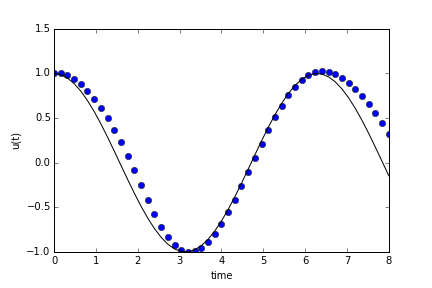
\includegraphics[width=2.5in]{euler50.png}\hfil
\hfil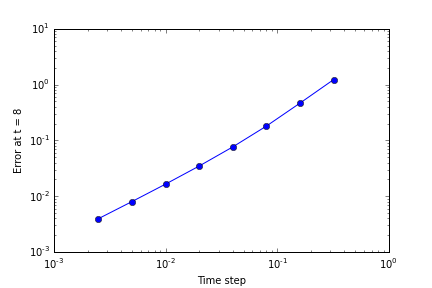
\includegraphics[width=2.5in]{euler_errors.png}\hfil
\caption{\label{fig:plots1} 
Left: the Euler solution with $N=50$, Right: Log-log plot of the error in
Forward Euler.
  }
\end{figure}


% uncomment the next two lines if you want to insert solution...
%\vskip 1cm
%{\bf Solution:}

% insert your solution here!




\end{document}

